% !TeX spellcheck = en_US
%\documentclass[11pt,a4paper]{article}
\documentclass[11pt
  , a4paper
  , article
  , oneside
%  , twoside
%  , draft
]{memoir}

\usepackage{control}
\usepackage[numbers]{natbib}


\begin{document}

\newcommand{\technumber}{
  RAON Control-Document Series\\
  Revision : v1.0,   Release : 2015-03-16 fixed date}
\title{\textbf{SRF Test Facility - Storage 시스템 구성}}

\author{이상일\thanks{silee7103@ibs.re.kr}, 이정한, 손창욱, 손형주, 박미정, 남승희 \\

  Rare Isotope Science Project\\
  Institute for Basic Science, Daejeon, South Korea
}
\date{\today}

\renewcommand{\maketitlehooka}{\begin{flushright}\textsf{\technumber}\end{flushright}}
%\renewcommand{\maketitlehookb}{\centering\textsf{\subtitle}}
%\renewcommand{\maketitlehookc}{C}
%\renewcommand{\maketitlehookd}{D}

\maketitle

\begin{abstract}
RAON is a particle accelerator to research the interaction between the nucleus forming a rare isotope as Korean heavy-ion accelerator. RAON accelerator consists of a number of facilities and equipments as a large-scaled experimental device operating under the distributed environment. 

ECR Ion source 및 RFQ Test를 위하여 문지동 카이스트 캠퍼스에 마련되 SRF Test Facility 건물에는 해당 장치의 Test시 발생하는 EPICS IOC 데이터를 저장하기 위한 목적으로 Storage 시스템이 구축되었다. 본 스토리지 시스템은 본 사이트에서 운영될 스토리지 시스템과 유사한 목적으로 가속기 실운영 환경하에서 스토리지 시스템은 운영 및 데이터 저장 성능에 대한 검증을 목적으로 한다. 본 문서에서는 SRF Test Facility 에서 운영될 스토리지 시스템의 구성에 대하여 상세 기술한다.

\end{abstract}

FPGA(Field Programmable Gate Array)는 Hardware의 IC 소자의 gate array를 사용자가 program하여 회로를 구성할 수 있는 chip을 말한다. FPGA 프로그램 개발은 HDL(Hardware Description Language) 개발표준 언어를 사용하며 프로그램 할 수 있으며 아래와 같은 두 가지 HDL 언어를 지원한다.

\begin{itemize}
	\item VHDL
	\item Verilog HDL
\end{itemize}

본 문서에는 Xilinx의 FPGA Chip 중 Zynq 사용을 위한 내용을 기술한다. Zynq의 특징은 앞서 설명한 FPGA의 특징과 ARM CPU를 내장한 embedded 특징 모두 가지는 하나의 SoC(System on Chip) 이다.  따라서 Zynq Chip에는 기존 FPGA에 가지는 장점에 embedded 형태의 운영체제를 가질 수 있는 장점이 있다. 또한 이 둘간의 interface는 AXI Bus interface를 통한 메모리 맵을 통하여 데이터 통신이 가능하다. 따라서 고속 신호처리를 위하여는 FPGA I/O를 low level(hardware) 단에서 처리를 하며, 상위 레벨과의 인터페이스 및 주요 제어로직은 CPU 모듈에서 처리 할 수 있는 설계가 가능하다. 이는 가속기 제어 operation sequence에 따른 timing event의 external trigger를 입력으로 받아 고속의 신호를 처리하여야 하는 application에 활용 할 수 있다. 또한 MPS(Machine Protection System)와 같은 고속의 application에 적용할 수 있으리라 판단된다.
Zynq는 ARM 계열의 CPU를 가지고 있으며 여기에 linux 운영체제를 쉽게 올릴 수 있는 petalinux softeware tool을 제공한다. 


\begin{lstlisting}[style=termstyle]
Switch Information Report for SW300


List of Switches

Switch ID   Worldwide Name           Enet IP Addr    FC IP Addr      Name
-------------------------------------------------------------------------
1: fffc01 10:00:00:27:f8:df:f3:c8 192.168.1.53    0.0.0.0        >"SW300"


Current Switch Information

Ethernet IP Address: 192.168.1.53
Ethernet Subnetmask: 255.255.255.0
Fibre Channel IP Address: 0.0.0.0
Fibre Channel Subnetmask: 0.0.0.0
Gateway Address: 192.168.1.1
Ethernet IPv6 Addresses: 

Kernel:     2.6.14.2   
Fabric OS:  v7.1.0a
Made on:    Tue Jan 22 19:37:11 2013
Flash:	    Thu Jan 30 19:54:48 2014
BootProm:   1.0.10
List of Inter-Switch Links

Local Domain ID: 1

Local Port     Domain     Remote Port     State
-------------------------------------------------------
List of Ports

switchName:	SW300
switchType:	71.2
switchState:	Online   
switchMode:	Native
switchRole:	Principal
switchDomain:	1
switchId:	fffc01
switchWwn:	10:00:00:27:f8:df:f3:c8
zoning:		ON (sw300)
switchBeacon:	OFF

Index Port Address Media Speed       State   Proto
==================================================
0   0   010000   id    N8	   Online      FC  F-Port  1 N Port + 1 NPIV public 
1   1   010100   id    N8	   Online      FC  F-Port  1 N Port + 1 NPIV public 
2   2   010200   id    N8	   Online      FC  F-Port  21:00:00:24:ff:4a:b8:b8 
3   3   010300   id    N8	   No_Light    FC  
4   4   010400   id    N8	   No_Light    FC  
5   5   010500   id    N8	   No_Light    FC  
6   6   010600   id    N8	   No_Light    FC  
7   7   010700   id    N8	   No_Light    FC  
8   8   010800   id    N8	   Online      FC  F-Port  1 N Port + 1 NPIV public 
9   9   010900   id    N8	   Online      FC  F-Port  1 N Port + 1 NPIV public 
10  10   010a00   id    N8	   Online      FC  F-Port  21:00:00:24:ff:4a:b8:b9 
11  11   010b00   id    N8	   No_Light    FC  
12  12   010c00   id    N8	   No_Light    FC  
13  13   010d00   id    N8	   No_Light    FC  
14  14   010e00   id    N8	   No_Light    FC  
15  15   010f00   id    N8	   No_Light    FC  
16  16   011000   --    N8	   No_Module   FC  (No POD License) Disabled
17  17   011100   --    N8	   No_Module   FC  (No POD License) Disabled
18  18   011200   --    N8	   No_Module   FC  (No POD License) Disabled
19  19   011300   --    N8	   No_Module   FC  (No POD License) Disabled
20  20   011400   --    N8	   No_Module   FC  (No POD License) Disabled
21  21   011500   --    N8	   No_Module   FC  (No POD License) Disabled
22  22   011600   --    N8	   No_Module   FC  (No POD License) Disabled
23  23   011700   --    N8	   No_Module   FC  (No POD License) Disabled
Name Server

{
010000 010001 010100 010101 010200 010800 010801 010900 
010901 010a00 
10 Nx_Ports in the Fabric } 

{
Type Pid    COS     PortName                NodeName                 TTL(sec)
N    010000;      3;50:00:d3:10:00:86:d6:05;50:00:d3:10:00:86:d6:00; na
FC4s: FCP 
PortSymb: [90] "Compellent Port QLGC FC 8Gbps; Slot=01 Port=01 in Controller: SN 34518 of Storage Center: "
NodeSymb: [47] "Compellent Storage Center: Storage Center 34518"
Fabric Port Name: 20:00:00:27:f8:df:f3:c8 
Permanent Port Name: 50:00:d3:10:00:86:d6:05
Port Index: 0
Share Area: No
Device Shared in Other AD: No
Redirect: No 
Partial: No
LSAN: No
N    010001;      3;50:00:d3:10:00:86:d6:1f;50:00:d3:10:00:86:d6:01; na
FC4s: FCP 
PortSymb: [110] "Compellent Port QLGC FC 8Gbps; Slot=01 Port=01 in Controller: SN 34518 of Storage Center: Storage Center 34518"
NodeSymb: [47] "Compellent Storage Center: Storage Center 34518"
Fabric Port Name: 20:00:00:27:f8:df:f3:c8 
Permanent Port Name: 50:00:d3:10:00:86:d6:05
Port Index: 0
Share Area: No
Device Shared in Other AD: No
Redirect: No 
Partial: No
LSAN: No
N    010100;      3;50:00:d3:10:00:86:d6:12;50:00:d3:10:00:86:d6:00; na
FC4s: FCP 
PortSymb: [110] "Compellent Port QLGC FC 8Gbps; Slot=01 Port=01 in Controller: SN 34519 of Storage Center: Storage Center 34518"
NodeSymb: [47] "Compellent Storage Center: Storage Center 34518"
Fabric Port Name: 20:01:00:27:f8:df:f3:c8 
Permanent Port Name: 50:00:d3:10:00:86:d6:12
Port Index: 1
Share Area: No
Device Shared in Other AD: No
Redirect: No 
Partial: No
LSAN: No
N    010101;      3;50:00:d3:10:00:86:d6:21;50:00:d3:10:00:86:d6:02; na
FC4s: FCP 
PortSymb: [110] "Compellent Port QLGC FC 8Gbps; Slot=01 Port=01 in Controller: SN 34519 of Storage Center: Storage Center 34518"
NodeSymb: [47] "Compellent Storage Center: Storage Center 34518"
Fabric Port Name: 20:01:00:27:f8:df:f3:c8 
Permanent Port Name: 50:00:d3:10:00:86:d6:12
Port Index: 1
Share Area: No
Device Shared in Other AD: No
Redirect: No 
Partial: No
LSAN: No
N    010200;      3;21:00:00:24:ff:4a:b8:b8;20:00:00:24:ff:4a:b8:b8; na
FC4s: FCP 
NodeSymb: [37] "QLE2562 FW:v5.04.01 DVR:v8.03.07.12-k"
Fabric Port Name: 20:02:00:27:f8:df:f3:c8 
Permanent Port Name: 21:00:00:24:ff:4a:b8:b8
Port Index: 2
Share Area: No
Device Shared in Other AD: No
Redirect: No 
Partial: No
LSAN: No
N    010800;      3;50:00:d3:10:00:86:d6:06;50:00:d3:10:00:86:d6:00; na
FC4s: FCP 
PortSymb: [90] "Compellent Port QLGC FC 8Gbps; Slot=01 Port=02 in Controller: SN 34518 of Storage Center: "
NodeSymb: [47] "Compellent Storage Center: Storage Center 34518"
Fabric Port Name: 20:08:00:27:f8:df:f3:c8 
Permanent Port Name: 50:00:d3:10:00:86:d6:06
Port Index: 8
Share Area: No
Device Shared in Other AD: No
Redirect: No 
Partial: No
LSAN: No
N    010801;      3;50:00:d3:10:00:86:d6:20;50:00:d3:10:00:86:d6:01; na
FC4s: FCP 
PortSymb: [110] "Compellent Port QLGC FC 8Gbps; Slot=01 Port=02 in Controller: SN 34518 of Storage Center: Storage Center 34518"
NodeSymb: [47] "Compellent Storage Center: Storage Center 34518"
Fabric Port Name: 20:08:00:27:f8:df:f3:c8 
Permanent Port Name: 50:00:d3:10:00:86:d6:06
Port Index: 8
Share Area: No
Device Shared in Other AD: No
Redirect: No 
Partial: No
LSAN: No
N    010900;      3;50:00:d3:10:00:86:d6:13;50:00:d3:10:00:86:d6:00; na
FC4s: FCP 
PortSymb: [110] "Compellent Port QLGC FC 8Gbps; Slot=01 Port=02 in Controller: SN 34519 of Storage Center: Storage Center 34518"
NodeSymb: [47] "Compellent Storage Center: Storage Center 34518"
Fabric Port Name: 20:09:00:27:f8:df:f3:c8 
Permanent Port Name: 50:00:d3:10:00:86:d6:13
Port Index: 9
Share Area: No
Device Shared in Other AD: No
Redirect: No 
Partial: No
LSAN: No
N    010901;      3;50:00:d3:10:00:86:d6:22;50:00:d3:10:00:86:d6:02; na
FC4s: FCP 
PortSymb: [110] "Compellent Port QLGC FC 8Gbps; Slot=01 Port=02 in Controller: SN 34519 of Storage Center: Storage Center 34518"
NodeSymb: [47] "Compellent Storage Center: Storage Center 34518"
Fabric Port Name: 20:09:00:27:f8:df:f3:c8 
Permanent Port Name: 50:00:d3:10:00:86:d6:13
Port Index: 9
Share Area: No
Device Shared in Other AD: No
Redirect: No 
Partial: No
LSAN: No
N    010a00;      3;21:00:00:24:ff:4a:b8:b9;20:00:00:24:ff:4a:b8:b9; na
FC4s: FCP 
NodeSymb: [37] "QLE2562 FW:v5.04.01 DVR:v8.03.07.12-k"
Fabric Port Name: 20:0a:00:27:f8:df:f3:c8 
Permanent Port Name: 21:00:00:24:ff:4a:b8:b9
Port Index: 10
Share Area: No
Device Shared in Other AD: No
Redirect: No 
Partial: No
LSAN: No
The Local Name Server has 10 entries }
Zoning Information

Defined configuration:
cfg:	sw300	SC4020_FD01_P_ALL; SC4020_FD01_V_ALL; 
SC4020_FD01_V_ALL_srfdb_S6_P1; SC4020_FD02_P_ALL; 
SC4020_FD02_V_ALL; SC4020_FD02_V_ALL_srfdb_S6_P2
zone:	SC4020_FD01_P_ALL	
SC4020_C0_P1; SC4020_C1_P1
zone:	SC4020_FD01_V_ALL	
SC4020_C0_V1; SC4020_C1_V1
zone:	SC4020_FD01_V_ALL_srfdb_S6_P1	
SC4020_C0_V1; SC4020_C1_V1; srfdb_S6_P1
zone:	SC4020_FD02_P_ALL	
SC4020_C0_P2; SC4020_C1_P2
zone:	SC4020_FD02_V_ALL	
SC4020_C0_V2; SC4020_C1_V2
zone:	SC4020_FD02_V_ALL_srfdb_S6_P2	
SC4020_C0_V2; SC4020_C1_V2; srfdb_S6_P2
alias:	SC4020_C0_P1	
50:00:d3:10:00:86:d6:05
alias:	SC4020_C0_P2	
50:00:d3:10:00:86:d6:06
alias:	SC4020_C0_V1	
50:00:d3:10:00:86:d6:1f
alias:	SC4020_C0_V2	
50:00:d3:10:00:86:d6:20
alias:	SC4020_C1_P1	
50:00:d3:10:00:86:d6:12
alias:	SC4020_C1_P2	
50:00:d3:10:00:86:d6:13
alias:	SC4020_C1_V1	
50:00:d3:10:00:86:d6:21
alias:	SC4020_C1_V2	
50:00:d3:10:00:86:d6:22
alias:	srfdb_S6_P1	
21:00:00:24:ff:4a:b8:b8
alias:	srfdb_S6_P2	
21:00:00:24:ff:4a:b8:b9

Effective configuration:
cfg:	sw300	
zone:	SC4020_FD01_P_ALL	
50:00:d3:10:00:86:d6:05
50:00:d3:10:00:86:d6:12
zone:	SC4020_FD01_V_ALL	
50:00:d3:10:00:86:d6:1f
50:00:d3:10:00:86:d6:21
zone:	SC4020_FD01_V_ALL_srfdb_S6_P1	
50:00:d3:10:00:86:d6:1f
50:00:d3:10:00:86:d6:21
21:00:00:24:ff:4a:b8:b8
zone:	SC4020_FD02_P_ALL	
50:00:d3:10:00:86:d6:06
50:00:d3:10:00:86:d6:13
zone:	SC4020_FD02_V_ALL	
50:00:d3:10:00:86:d6:20
50:00:d3:10:00:86:d6:22
zone:	SC4020_FD02_V_ALL_srfdb_S6_P2	
50:00:d3:10:00:86:d6:20
50:00:d3:10:00:86:d6:22
21:00:00:24:ff:4a:b8:b9

SFP Serial ID Information

Port  0: id (sw) Vendor: BROCADE          Serial No: UAF414260001WGM  Speed: 2,4,8_Gbps 
Port  1: id (sw) Vendor: BROCADE          Serial No: UAF414260001WC5  Speed: 2,4,8_Gbps 
Port  2: id (sw) Vendor: BROCADE          Serial No: UAF414260001WFT  Speed: 2,4,8_Gbps 
Port  3: id (sw) Vendor: BROCADE          Serial No: UAF414260001WM4  Speed: 2,4,8_Gbps 
Port  4: id (sw) Vendor: BROCADE          Serial No: UAF414260001WGK  Speed: 2,4,8_Gbps 
Port  5: id (sw) Vendor: BROCADE          Serial No: UAF414260001WGU  Speed: 2,4,8_Gbps 
Port  6: id (sw) Vendor: BROCADE          Serial No: UAF414260001WEV  Speed: 2,4,8_Gbps 
Port  7: id (sw) Vendor: BROCADE          Serial No: UAF414260001WDD  Speed: 2,4,8_Gbps 
Port  8: id (sw) Vendor: BROCADE          Serial No: UAF41420000026E  Speed: 2,4,8_Gbps 
Port  9: id (sw) Vendor: BROCADE          Serial No: UAF41420000024A  Speed: 2,4,8_Gbps 
Port 10: id (sw) Vendor: BROCADE          Serial No: UAF41420000026W  Speed: 2,4,8_Gbps 
Port 11: id (sw) Vendor: BROCADE          Serial No: UAF414200000258  Speed: 2,4,8_Gbps 
Port 12: id (sw) Vendor: BROCADE          Serial No: UAF41420000024P  Speed: 2,4,8_Gbps 
Port 13: id (sw) Vendor: BROCADE          Serial No: UAF41420000024Z  Speed: 2,4,8_Gbps 
Port 14: id (sw) Vendor: BROCADE          Serial No: UAF41420000026B  Speed: 2,4,8_Gbps 
Port 15: id (sw) Vendor: BROCADE          Serial No: UAF41420000024V  Speed: 2,4,8_Gbps 
Port 16: -- 
Port 17: -- 
Port 18: -- 
Port 19: -- 
Port 20: -- 
Port 21: -- 
Port 22: -- 
Port 23: -- 
\end{lstlisting}

\clearpage

\chapter{Storage System}

\section{특성}

\begin{figure}[h!]
	\centering
	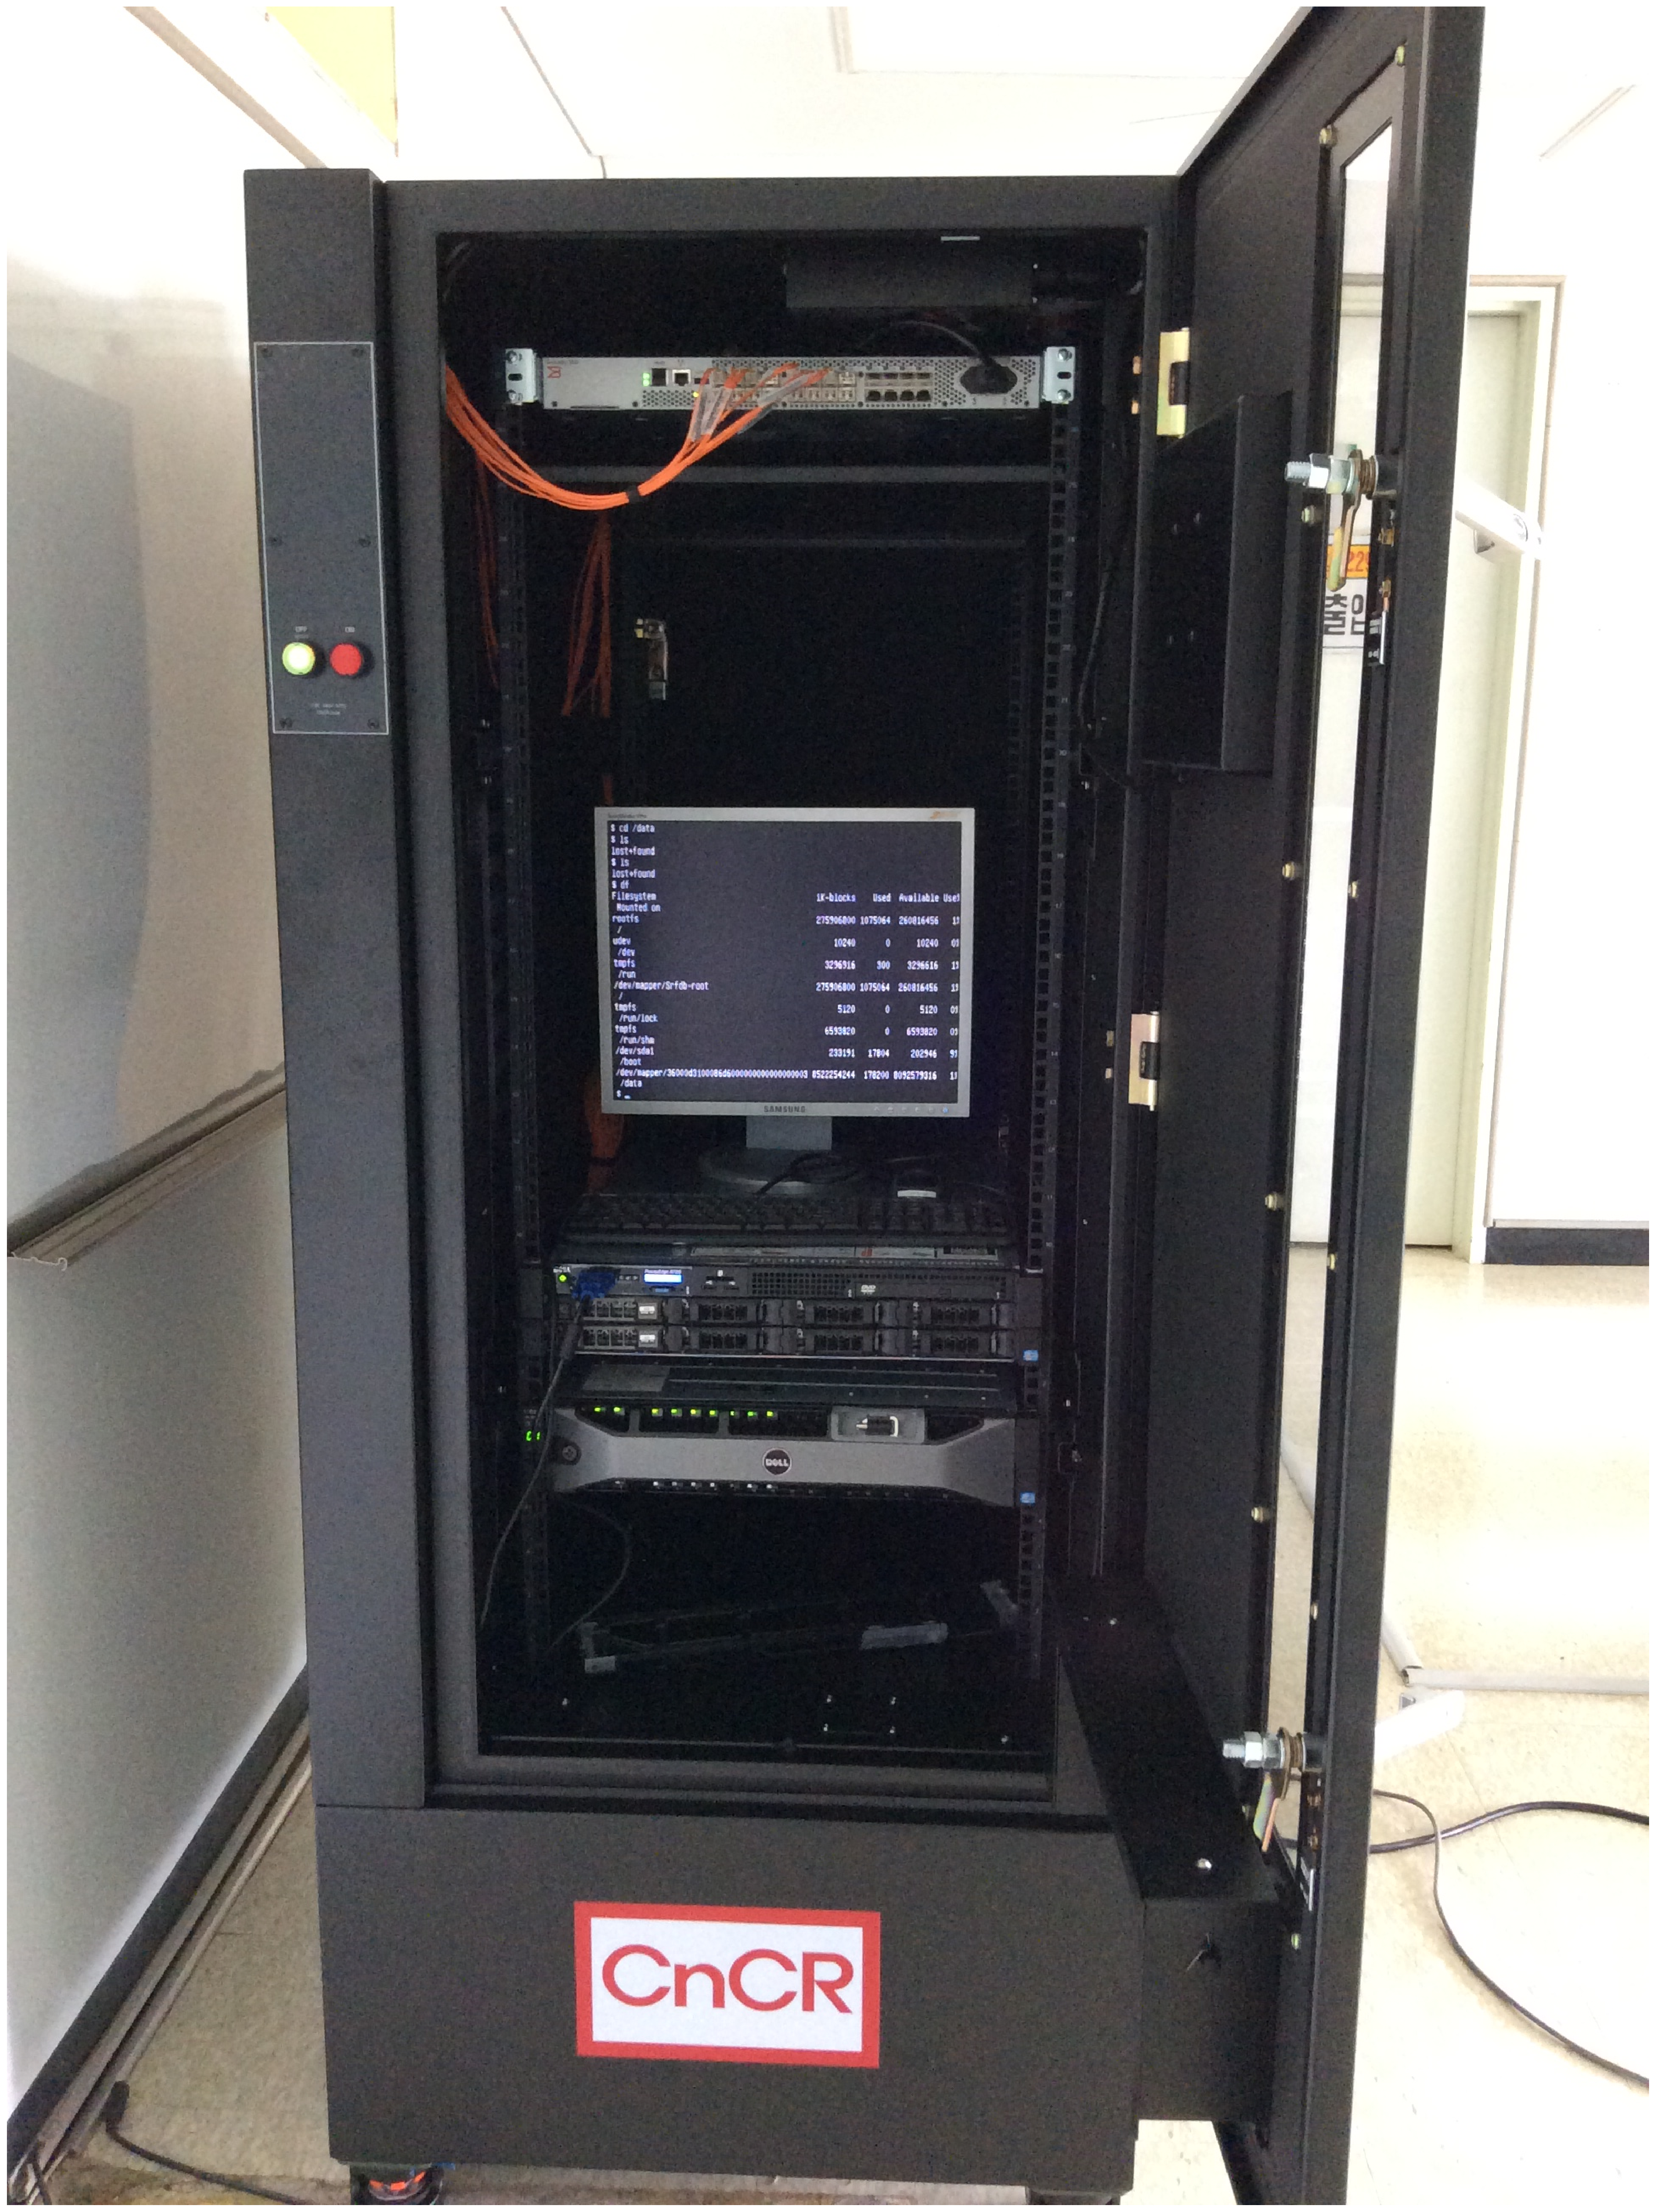
\includegraphics[width=0.85\textwidth]{./images/srfdb_fore.eps}
	\caption{SRF Storage 시스템 전면}
	\label{fig:srfdb_fore} 
\end{figure}


\clearpage

\bibliographystyle{unsrtnat}
\bibliography{./refs}

\end{document}

